\documentclass[conference]{llncs}
% The preceding line is only needed to identify funding in the first footnote. If that is unneeded, please comment it out.
\usepackage{cite}
\usepackage{amsmath,amssymb,amsfonts}
\usepackage{algorithmic}
\usepackage{graphicx}
\usepackage{dblfloatfix}

\def\BibTeX{{\rm B\kern-.05em{\sc i\kern-.025em b}\kern-.08em
    T\kern-.1667em\lower.7ex\hbox{E}\kern-.125emX}}
    
\begin{document}

\title{Bayesian Learning of Finite Asymmetric Gaussian Mixtures}

\author{Shuai Fu\inst{1} \and Nizar Bouguila\inst{2}}

\institute{Concordia University, Montreal, Canada. \textbf{Email:} \email{f\_shuai@encs.concordia.ca}
\and Concordia University, Montreal, Canada. \textbf{Email:} \email{bouguila@ciise.concordia.ca} }


\maketitle

\begin{abstract}
Asymmetric Gaussian mixture (AGM) model has been proven to be more flexible than the classic Gaussian mixture model from many aspects. In contrast with previous efforts that have focused on maximum likelihood estimation, this paper introduces a fully Bayesian learning approach using Metropolis-Hastings (MH) within Gibbs sampling method to learn AGM model. We show the merits of the proposed model using synthetic data and a challenging intrusion detection application.
\bigbreak
\textbf{Keywords - Asymmetric Gaussian Mixture, Metropolis-Hastings, Gibbs Sampling, MCMC, Intrusion Detection}
\end{abstract}

\section{Introduction}
A large volume of data is generated everyday. A crucial task is the analysis and modeling of these data. Many statistical and data mining approaches have been proposed in the past. Among these approaches, finite mixture models \cite{Bouguila2005,Bouguila2007,Sefidpour2012,Bouguila2009a} have received a lot of attention because they are flexible and powerful probabilistic tools for modeling data \cite{McLachlan2000}. In recent years, there has been an increasing trend of applying finite mixtures into unsupervised learning domains involving statistical modeling of data, such as astronomy, ecology, bioinformatics, pattern recognition, computer vision and machine learning \cite{Bouguila2006}. As an improvement of naive Bayes methodologies, mixture modeling can be viewed as the superimposition of a finite number of component densities which respects the dependency between data groups, bringing more generality and robustness. 

As an efficient approach, Gaussian mixture model (GMM) \cite{Elguebaly2010} is widely deployed because of its outstanding suitability in several domains such as computer vision, pattern recognition and data mining. In this paper, we choose asymmetric Gaussian mixture (AGM) model \cite{Elguebaly2014} for modeling because it uses two variance parameters for left and right parts of each distribution in the mixture which allows to accurately model non-Gaussian datasets \cite{Bouguila2012a,Boutemedjet2010} including asymmetric ones. 

A challenging issue when deploying mixture models is the learning of the model's parameters. The estimation of the parameters of mixture distributions can be accomplished by using maximum-likelihood-based expectation maximization (EM) \cite{Dempster1977} algorithm. However, EM has some drawbacks such as overfitting and dependency on initialization \cite{Bouguila2005a,Bouguila2009,Bouguila2012}. Therefore, an alternative is the fully Bayesian approach, based for instance on Markov Chain Monte Carlo (MCMC) methods \cite{Hastings1970}, which has been found to be useful in many applications by considering parameters priors which can avoid overfitting problems. As a sampling-based learning approach, the main difficulty of MCMC method is that, under some circumstances, direct sampling is not always straightforward. As widely deployed implementations of MCMC method, Metropolis-Hastings (Hastings, 1970)\cite{Hastings1970} and Gibbs sampling (Bouguila, N., 2011) \cite{Bouguila2011} methods can be introduced to solve this problem through applying proposal priors and posteriors and sampling one parameter by giving the others. By combining the advantages of both sampling techniques together, the Metopolis-Hastings within Gibbs method \cite{Bouguila2009} \cite{Bourouis2014} is selected as the learning algorithm for AGM model.

The rest of this paper is organized as follows. Section 2 illustrates the AGM model and its Bayesian learning process. Section 3 is devoted to experimental results using both synthetic data and a real application (network intrusion detection). Finally, Section 4 concludes the paper.

\section{Bayesian Model}
\subsection{Asymmetric Gaussian Mixture Model}
Assuming that the AGM model has $M$ components then the likelihood function (Elguebaly and Bouguila, 2013)\cite{Elguebaly2014} is defined as follows:
\begin{align}
p(\mathcal{X}|\Theta) = \prod_{i=1}^N \sum_{j=1}^Mp_jp(X_i|\xi_j)
\label{eq:1}
\end{align}
where $\mathcal{X} = (X_1,...,X_N)$ is the set of $N$ observations, $\Theta = \{p_1,...,p_M, \xi_1,...,\xi_M\}$ represents the parameters set, $p_j$ (0 $< p_j \leq$ 1 and $\sum_{j=1}^Mp_j$ = 1) is the weight for each component in the mixture model and $\xi_j$ is the AGD parameters of mixture component $j$. Giving $X = (x_1,...,x_d)$, the probability density function (Elguebaly and Bouguila, 2013)\cite{Elguebaly2014} can be defined as follows:
\begin{align}
p(X|\xi_j) \propto \prod_{k=1}^{d} \frac{1}{(\sigma_{l_{jk}}+\sigma_{r_{jk}})}
\times \left\{\begin{matrix}
\exp \begin{bmatrix}
-\frac{(x_k-\mu_{jk})^2}{2(\sigma_{l_{jk}})^2}
\end{bmatrix}\ if\ x_k\ <\ \mu_{jk} \\ 
\exp \begin{bmatrix}
-\frac{(x_k-\mu_{jk})^2}{2(\sigma_{r_{jk}})^2}
\end{bmatrix}\ if\ x_k\ \geqslant\ \mu_{jk} \\ 
\end{matrix}\right.
\label{eq:2}
\end{align}
where $\xi_j = (\mu_j,\sigma_{lj},\sigma_{rj})$ is the set of parameters of component $j$ and $\mu_j = (\mu_{j1},...,\mu_{jd})$ is the mean, $\sigma_{lj} = (\sigma_{lj1},...,\sigma_{ljd})$ and $\sigma_{rj} = (\sigma_{rj1},...,\sigma_{rjd})$ are the left and right standard deviations for AGD. To be more specific, $x_k \thicksim N(\mu_{jk},\sigma_{ljk})\ (x_k < \mu_{jk})$ and $x_k \thicksim N(\mu_{jk},\sigma_{rjk})\ (x_k \geqslant \mu_{jk})$ for each dimension.

In order to simplify the Bayesian learning process, we introduce a $M$-dimensio-nal membership vector $Z$ for each observation $X_i, 1 < i <N, Z_i = (Z_{i1},...,Z_{iM})$ which indicates to which specific component $X_i$ belongs (Bouguila, Ziou and Monga, 2006)\cite{Bouguila2006}, such that:
\begin{align}
Z_{ij} = \left\{\begin{matrix}
1\qquad\mbox{ if }X_i\mbox{  belongs to component }j \\
0\qquad\quad\qquad \mbox{otherwise} \qquad\qquad\quad\quad \\
\end{matrix}\right.
\label{eq:3}
\end{align}
in other words, $Z_{ij} = 1$ only if observation $X_i$ has the highest probability of belonging to component $j$ and accordingly, for other components, $Z_{ij} = 0$. 

By combining Eq. \eqref{eq:1} and Eq. \eqref{eq:3} together we derive the complete likelihood function:
\begin{align}
p(\mathcal{X}, Z|\Theta) = \prod_{i=1}^{N}\prod_{j=1}^{M}(p_jp(X_i|\xi_j))^{Z_{ij}}
\label{eq:4}
\end{align}

\subsection{Learning Algorithm}
Before describing MH-within-Gibbs learning steps, the priors and posteriors need to be specified. First, we denote the postorior probability of membership vector Z as $\pi(Z|\Theta,\mathcal{X})$ (Elguebaly and Bouguila, 2011)\cite{Elguebaly2011}:
\begin{align}
Z^{(t)} \sim \pi(Z|\Theta^{(t-1)},\mathcal{X})
\label{eq:5}
\end{align}
the number of observations belonging to a specific component $j$ can be calculated using $Z^{(t)}$ as follows:
\begin{align}
n_j^{(t)} = \sum_{i=1}^NZ_{ij}\ (j = 1,...,M) 
\label{eq:6}
\end{align}
thus $n^{(t)}=(n_i^{(t)},...,n_M^{(t)})$ represents the number of observations belonging to each mixture component.

Since the mixture weight $p_j$ satisfies the following conditions (0 $< p_j \leq$ 1 and $\sum_{j=1}^Mp_j$ = 1), a natural choice of the prior is Dirichlet distribution as follows \cite{Bouguila2004} \cite{Bouguila2004a} 
\begin{align}
\pi(p_j^{(t)}) \sim \mathcal{D}(\gamma_1,...,\gamma_M )
\label{eq:7}
\end{align}
where $\gamma_j$ is known hyperparameter. Consequently, the posterior of the mixture weight $p_j$ is:
\begin{align}
p(p_j^{(t)}|Z^{(t)}) \sim \mathcal{D}(\gamma_1 + n_1^{(t)},...,\gamma_M + n_M^{(t)})
\label{eq:8}
\end{align}


Direct sampling of mixture parameters $\xi \sim p(\xi|Z,\mathcal{X})$ could be difficult so Metropolis-Hastings method should be deployed using proposal distributions for $\xi^{(t)} \sim q(\xi|\xi^{(t-1)})$. To be more specific, for parameters of AGM model which are $\mu$ , $\sigma_l$ and $\sigma_r$, we choose proposal distributions as follows:
\begin{align}
\mu_j^{(t)} \sim \mathcal{N}_d(\mu_j^{(t-1)},\Sigma)
\label{eq:9}
\end{align}
\begin{align}
\sigma_{lj}^{(t)} \sim \mathcal{N}_d(\sigma_{lj}^{(t-1)},\Sigma)
\label{eq:10}
\end{align}
\begin{align}
\sigma_{rj}^{(t)} \sim \mathcal{N}_d(\sigma_{rj}^{(t-1)},\Sigma)
\label{eq:11}
\end{align}
the proposal distributions are $d$-dimensional Gaussian distributions with $\Sigma$ as $d$ x $d$ identity matrix which makes the sampling a random walk MCMC process.

As the most important part of Metropolis-Hastings method, at the end of each iteration, for new generated mixture parameter set $\Theta^{(t)}$, an acceptance ratio $r$ needs to be calculated in order to make a decision whether they should be accepted or discarded for the next iteration. The acceptance ratio $r$ is given by:
\begin{align}
r = \frac{p(\mathcal{X}|\Theta^{(t)})\pi(\Theta^{(t)})q(\Theta^{(t-1)}|\Theta^{(t)})}{p(\mathcal{X}|\Theta^{(t-1)})\pi(\Theta^{(t-1)})q(\Theta^{(t)}|\Theta^{(t-1)})}
\label{eq:12}
\end{align}

where $\pi(\Theta)$ is the proposed prior distribution which can be decomposed to $d$-dimensional Gaussian distributions such that $\mu \sim \mathcal{N}_d(\eta,\Sigma)$ and $\sigma_l, \sigma_r \sim \mathcal{N}_d(\tau,\Sigma)$ given known hyperparameters $\eta$ and $\tau$. Since mixture weight $p$ has been computed previously during the Gibbs sampling part, it should not be included in Eq. \eqref{eq:12}. Further information about the calculation of acceptance ratio $r$ is explained in Appendix A.

Once acceptance ratio $r$ is derived by Eq. \eqref{eq:15}, we compute acceptance probability $\alpha = min[1,r]$ \cite{Luengo2013}. Then $u \sim U_{[0,1]}$ is supposed to be generated randomly. If $\alpha < u$, the proposed move should be accepted and parameters should be updated by $p^{(t)}$ and $\xi^{(t)}$ for next iteration. Otherwise, we discard $p^{(t)}$, $\xi^{(t)}$ and set $p^{(t)} = p^{(t-1)}$, $\xi^{(t)} = \xi^{(t-1)}$.

We summarize the MH-within-Gibbs learning process for AGM model in the following steps:
\bigbreak
\noindent\textbf{Input:} Data observations $\mathcal{X}$ and components number $M$ \\
\textbf{Output:} AGM mixture parameter set $\Theta$
\bigbreak

\begin{enumerate}
\item Initialization
\item Step $t$: For $t = 1,\ldots$
\begin{enumerate}
\item[]\textbf{Gibbs sampling part}
\item Generate $Z^{(t)}$ from Eq. \eqref{eq:5}
\item Compute $n_j^{(t)}$ from Eq. \eqref{eq:6}
\item Generate $p_j^{(t)}$ from Eq. \eqref{eq:8}
\item[] \textbf{Metropolis-Hastings part}
\item Sample $\xi_j^{(t)}$ ($\mu_j^{(t)}, \sigma_{lj}^{(t)}, \sigma_{rj}^{(t)}$) from Eqs. \eqref{eq:9} \eqref{eq:10} \eqref{eq:11}
\item Compute acceptance ratio $r$ from Eq. \eqref{eq:15}
\item Generate $\alpha = min[1,r]$ and $u \sim U_{[0,1]}$
\item If $\alpha \geq u$ then $\xi^{(t)} = \xi^{(t-1)}$
\end{enumerate}
\end{enumerate}
\bigskip

\section{Experimental Results}
\subsection{Design of Experiments}
We apply the AGM model to both synthetic data and intrusion detection. For synthetic data validation, testing observations will be generated from AGM with known components number $M$ and experimental results will be evaluated by comparing the estimated and actual mixture parameters. In intrusion detection application, we select NSL-KDD dataset \cite{Tavallaee2009} as testing database. K-means algorithm is used for initialization and the results analysis will be based on statistics derived from confusion matrix.

\subsection{Synthetic Data}
The main goals of this section are feasibility analysis and efficiency evaluation of the AGM learning algorithm. The number of observations is set to 300 grouped into two clusters ($M$ = 2). Hyperparameters are set to $\gamma_j = 1$ \cite{Stephens2000} for sampling mixture weight $p_j$ from Eq. \eqref{eq:8}. $\eta$ and $\tau$ are considered as $d$-dimensional zero vectors in prior distributions of mixture parameter $\xi$.

Different proposed component numbers ($M' = 1,\dots,5$) are tested during the AGM learning process and the statistics are summarized in Table \ref{tab1}. In order to select the best number of components, we consider marginal likelihood as described in \cite{Bouguila2009}. The probability density functions are plotted for both original and estimated AGM components and the polylines show the trace of accepted moves for each component.

In terms of the best fit result, the accuracy is evaluated by calculating the Euclidean distance between original and estimated mixture parameter sets $\xi$ and $\hat{\xi}$ (Table \ref{tab2}). In summary, the estimation of mean is accurate because the Euclidean distance between $\mu_j$ and $\hat{\mu}_j$ is small but the distance between standard deviation $\sigma_{lj}, \sigma_{rj}$ and $\hat{\sigma}_{lj}, \hat{\sigma}_{rj}$ is slightly significant. However, this difference has not affected the clustering result.

 
\begin{table}
\caption{AGM Learning Statistics}
\begin{center}
\begin{tabular}{|c|c|c|c|}
\hline
\multicolumn{1}{|p{2cm}|}{\centering \textbf{Component number $M'$}} & \multicolumn{1}{|p{2cm}|}{\centering \textbf{\textit{Moves accepted}}} & \multicolumn{1}{|p{2cm}|}{\centering \textbf{\textit{Acceptance ratio}}} & \multicolumn{1}{|p{2cm}|}{\centering \textbf{\textit{Marginal likelihood}}}\\
\hline
1 & 22 & 7.33\% & -1596.143  \\
2 & 11 & 3.67\% & -1500.370 \\
3 & 14 & 4.67\% & -1684.518 \\
4 & 63 & 21.00\% & -1522.148 \\
5 & 39 & 13.00\% & -1517.533 \\
\hline
\end{tabular}
\label{tab1}
\end{center}
\end{table}

\bigskip

\begin{figure}
\centering
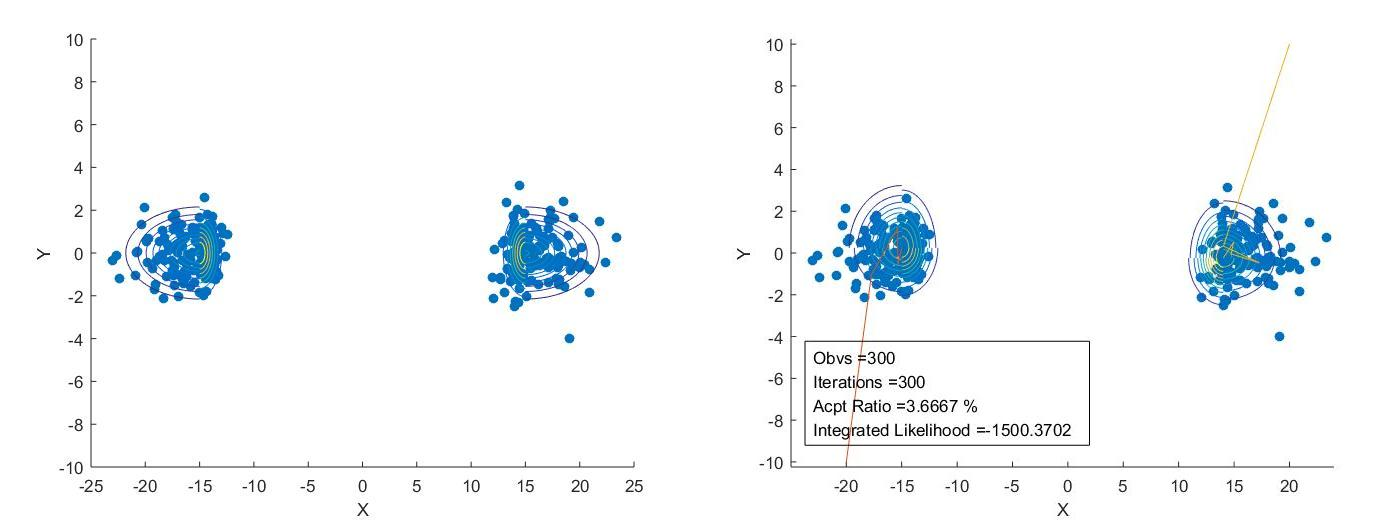
\includegraphics[width=0.6\paperwidth]{02.jpg}
\caption{Original synthetic observations and learning result ($M' = M = 2$)}
\label{fig:1}
\end{figure}

\bigskip

\begin{table}
\caption{Accuracy Analysis ($M' = M = 2$)}
\begin{center}
\begin{tabular}{|c|c|c|c|}
\hline
\multicolumn{1}{|p{3cm}|}{\centering \textbf{Component number $j = 1$}} & \multicolumn{1}{|p{2cm}|}{\centering \textbf{Mean \\($\mu_j$)}} & \multicolumn{1}{|p{3cm}|}{\centering \textbf{Left standard deviation ($\sigma_{lj}$)}} & \multicolumn{1}{|p{3cm}|}{\centering \textbf{Right standard deviation ($\sigma_{rj}$)}}\\
\hline
$\xi$ & [-15.00, 0.00] & [10.00, 1.00] & [1.00, 1.00]  \\
$\hat{\xi}$ & [-14.99, 0.25] & [4.77, 1.13] & [2.31, 1.88] \\
Euclidean Distance & 0.246 & 5.236 & 1.581 \\
\hline
\multicolumn{1}{|p{3cm}|}{\centering \textbf{Component number $j = 2$}} & \multicolumn{1}{|p{2cm}|}{\centering \textbf{Mean \\($\mu_j$)}} & \multicolumn{1}{|p{3cm}|}{\centering \textbf{Left standard deviation ($\sigma_{lj}$)}} & \multicolumn{1}{|p{3cm}|}{\centering \textbf{Right standard deviation ($\sigma_{rj}$)}}\\
\hline
$\xi$ & [15.00, 0.00] & [1.00, 1.00] & [10.00, 1.00]  \\
$\hat{\xi}$ & [14.02, -0.24] & [2.04, 1.04] & [5.70, 1.59] \\
Euclidean Distance & 1.010 & 1.036 & 4.338 \\
\hline
\end{tabular}
\label{tab2}
\end{center}
\end{table}

\subsection{Intrusion Detection}
Along with the development of information-based industries, network security problems are becoming increasingly important today. In order to address this challenge, many data mining methodologies were proposed including both classif-ication-based \cite{Puttini2003} and clustering-based \cite{Zhong2007} \cite{Fan2011} ones. However, classification-based solutions generally perform ineffectively for dynamic and variate attacking methods because changes of the intrusion patterns cannot be automatically adapted by supervised learning algorithms. Consequently, unsupervised approach such as AGM model is more favorable for modern intrusion-detection.

We select NSL-KDD \cite{Tavallaee2009}, an improved KDDCUP'99 intrusion-detection data-set, as the testing target since redundant records have been removed from original dataset to avoid potential learning bias. Before applying the testing models onto the dataset, the data pre-processing is needed since discrete enumerated values must be translated to numerical ones and be normalized properly to lead an accurate result. Therefore, we substitute enumerated values with their numbers of occurrences which could reflect the density distribution of discrete values. Having all numerical data in hand, we apply feature scaling method to normalize numerical values between 0 to 1 as follows:

\begin{align}
x' = \frac{x - min(x)}{max(x) - min(x)}
\label{eq:13}
\end{align}
where $x$ and $x'$ denote original and normalized values. In this way we could use unified proposal distribution for every dimension with the same value of hyperparameter $\Sigma$ during random walk MCMC sampling step (Table \ref{tab3}).

K-means clustering algorithm \cite{Hartigan1979} is chosen for the comparison of accuracy. Testing data records with total amount of 25192 (20\% of NSL-KDD dataset) are clustered into two groups with 11743 intrusions and 13449 normal behaviors indicating components number $M' = 2$. In order to better evaluate the pros and cons of models, results derived from Gaussian mixture model (GMM) will also be taken into consideration. The comparison based on confusion matrices resulted from K-means, GMM and AGM model (Table \ref{tab4}) reveals the fact that based on a less accurate initialization given by K-means (60.85\%), GMM performs almost the same way as K-means and the difference between these two models is trivial. In contrast, AGM model makes a significant improvement with much higher accuracy rate (80.47\%) and precision percentage (96.86\%), while much lower false positive rate (4.26\%) illustrating AGM model is capable of effectively detecting intrusions from background noises. Compared with K-means and GMM, AGM model has a higher false negative rate (28.58\%) which means it tends to strictly identify normal behaviors as intrusions which could be mitigated by reducing dimensions of dataset using feature selection methodologies.

%\begin{table}
%\caption{Original NSL-KDD data records}
%\begin{center}
%\begin{tabular}{|c|c|}
%\hline
%\multicolumn{1}{|p{1cm}|}{\centering\textbf{No}} & \multicolumn{1}{|p{10cm}|}{\centering\textbf{\textit{Value}}}\\
%\hline
%1 & {\tiny 0,tcp,ftp\_data,SF,491,0,0,0,0,0,0,0,0,0,0,0,0,0,0,0,0,0,2,2,0.00,0.00,0.00,0.00,1.00,0.00,0.00,150,25,0.17,0.03,0.17,0.00,0.00,0.00,0.05,0.00,normal}\\
%2 & {\tiny 0,udp,other,SF,146,0,0,0,0,0,0,0,0,0,0,0,0,0,0,0,0,0,13,1,0.00,0.00,0.00,0.00,0.08,0.15,0.00,255,1,0.00,0.60,0.88,0.00,0.00,0.00,0.00,0.00,normal} \\
%3 & {\tiny 0,tcp,private,S0,0,0,0,0,0,0,0,0,0,0,0,0,0,0,0,0,0,0,123,6,1.00,1.00,0.00,0.00,0.05,0.07,0.00,255,26,0.10,0.05,0.00,0.00,1.00,1.00,0.00,0.00,neptune} \\
%4 & {\tiny 0,tcp,http,SF,232,8153,0,0,0,0,0,1,0,0,0,0,0,0,0,0,0,0,5,5,0.20,0.20,0.00,0.00,1.00,0.00,0.00,30,255,1.00,0.00,0.03,0.04,0.03,0.01,0.00,0.01,normal} \\
%5 & {\tiny 0,tcp,http,SF,199,420,0,0,0,0,0,1,0,0,0,0,0,0,0,0,0,0,30,32,0.00,0.00,0.00,0.00,1.00,0.00,0.09,255,255,1.00,0.00,0.00,0.00,0.00,0.00,0.00,0.00,normal} \\
%6 & {\tiny 0,icmp,eco\_i,SF,18,0,0,0,0,0,0,0,0,0,0,0,0,0,0,0,0,0,1,1,0.00,0.00,0.00,0.00,1.00,0.00,0.00,1,16,1.00,0.00,1.00,1.00,0.00,0.00,0.00,0.00,ipsweep} \\
%\hline
%\end{tabular}
%\label{tab3}
%\end{center}
%\end{table}

\begin{table}
\caption{Translation and Normalization of Internet Protocols (Enumerated Values)}
\begin{center}
\begin{tabular}{|c|c|c|}
\hline
\multicolumn{1}{|p{2cm}|}{\centering \textbf{Internet Protocols}} & \multicolumn{1}{|p{2cm}|}{\centering \textbf{\textit{Number of Occurrences}}} & \multicolumn{1}{|p{2cm}|}{\centering \textbf{\textit{Normalized Values}}}\\
\hline
ICMP & 1655 & 0\\
UDP & 3011 & 0.071867 \\
TCP & 20526 & 1 \\
\hline
\end{tabular}
\label{tab3}
\end{center}
\end{table}

\begin{table}
\caption{Confusion Matrices and Statistics of K-means, GMM and AGM Models}
\begin{center}
\begin{minipage}{.3\textwidth}

\begin{center}
\textbf{K-means} \\
\begin{tabular}{|c|c|c|}
\hline
 & \multicolumn{1}{|p{1cm}|}{\centering \textbf{\textit{NF $^{\mathrm{a}}$}}} & \multicolumn{1}{|p{1cm}|}{\centering \textbf{\textit{F $^{\mathrm{b}}$}}}\\
\hline
\multicolumn{1}{|p{1cm}|}{\centering \textbf{\textit{NF}}} & 2445 & 9298\\
\multicolumn{1}{|p{1cm}|}{\centering \textbf{\textit{F}}} & 565 & 12884\\
\hline
\end{tabular}
\end{center}
\end{minipage}
\begin{minipage}{.3\textwidth}
    
\begin{center}
\textbf{GMM} \\
\begin{tabular}{|c|c|c|}
\hline
 & \multicolumn{1}{|p{1cm}|}{\centering \textbf{\textit{NF}}} & \multicolumn{1}{|p{1cm}|}{\centering \textbf{\textit{F}}}\\
\hline
\multicolumn{1}{|p{1cm}|}{\centering \textbf{\textit{NF}}} & 2464 & 9279\\
\multicolumn{1}{|p{1cm}|}{\centering \textbf{\textit{F}}} & 584 & 12865\\
\hline

\end{tabular}
\end{center}
\end{minipage}
\begin{minipage}{.3\textwidth}
    
\begin{center}
\textbf{AGM} \\
\begin{tabular}{|c|c|c|}
\hline
 & \multicolumn{1}{|p{1cm}|}{\centering \textbf{\textit{NF}}} & \multicolumn{1}{|p{1cm}|}{\centering \textbf{\textit{F}}}\\
\hline
\multicolumn{1}{|p{1cm}|}{\centering \textbf{\textit{NF}}} & 11484 & 259\\
\multicolumn{1}{|p{1cm}|}{\centering \textbf{\textit{F}}} & 5621 & 7828\\
\hline
\end{tabular}
\end{center}
\end{minipage}  
\end{center}
    
\begin{center}
\begin{tabular}{|c|c|c|c|}
\hline
& \multicolumn{1}{|p{2.5cm}|}{\centering \textbf{\textit{K-means}}} & \multicolumn{1}{|p{2.5cm}|}{\centering \textbf{\textit{GMM}}} & \multicolumn{1}{|p{2.5cm}|}{\centering \textbf{\textit{AGM}}}\\
\hline
\multicolumn{1}{|p{3.5cm}|}{\centering \textbf{\textit{Accuracy}}} & 60.85\% & 60.85\% & 76.66\%\\
\multicolumn{1}{|p{3.5cm}|}{\centering \textbf{\textit{Precision}}} & 20.82\% & 20.98\% & 97.79\%\\
\multicolumn{1}{|p{3.5cm}|}{\centering \textbf{\textit{False Positive Rate}}} & 41.92\% & 41.90\% & 3.20\%\\
\multicolumn{1}{|p{3.5cm}|}{\centering \textbf{\textit{False Negative Rate}}} & 18.77\% & 19.16\% & 32.86\%\\
\hline
\multicolumn{3}{l}{$^{\mathrm{a}}$Non fault-prone, $^{\mathrm{b}}$Fault-prone.}
\end{tabular}
\end{center}
\label{tab4}
\end{table}

\section{Conclusion and Future Work}
This paper illustrated a new intrusion detection approach by applying asymmetric Gaussian mixtures with a fully Bayesian learning process which is achieved by applying a hybrid sampling-based MH-within-Gibbs learning algorithm. According to the experiment results, the AGM model is proved as an effective approach for clustering.
In spite of the advantages of AGM we mentioned above, some improvements are still needed to promote the accuracy and flexibility and mitigate the drawbacks. Therefore, we plan to extend the Bayesian learning process and introduce model selection and feature selection methodologies to improve the performance in the case of high-dimensional datasets. The proposed work could be applied to other applications such as content-based images summarization \cite{Bouguila2007a}, retrieval \cite{Bouguila2004b}, and suggestion \cite{Boutemedjet2007}.

\section*{Appendix A}
\subsection{Derivation of Acceptance Ratio $r$ by Eq. \eqref{eq:12}}
The derivation of acceptance ratio $r$ is based on the assumption that mixture parameters are independent from each other which means that:
\bigskip
\begin{multline}
\qquad\qquad\pi(\Theta) = \pi(p,\xi) = \pi(\xi) \\
= \prod_{j=1}^M\pi(\mu_j)\pi(\sigma_{lj})\pi(\sigma_{rj}) \qquad\qquad\qquad\qquad\qquad\\
= \prod_{j=1}^M\mathcal{N}_d(\mu_j|\eta,\Sigma)\mathcal{N}_d(\sigma_{lj}|\tau,\Sigma)\mathcal{N}_d(\sigma_{rj}|\tau,\Sigma)\qquad\qquad\qquad
\label{eq:14}
\end{multline}
in Eq. \eqref{eq:14}, since the mixture weigh $p$ is generated following Gibbs sampling method whose acceptance ratio is always 1, it should be excluded from Metropolis-Hastings estimation step. Accordingly, apply the same rule to the proposal distribution as well:
\begin{multline}
\qquad\qquad q(\Theta^{(t)}|\Theta^{(t-1)}) = q(\xi^{(t)}|\xi^{(t-1)}) \\
= \prod_{j=1}^M\mathcal{N}_d(\mu_j^{(t)}|\mu_j^{(t-1)},\Sigma)\mathcal{N}_d(\sigma_{lj}^{(t)}|\sigma_{lj}^{(t-1)},\Sigma)\mathcal{N}_d(\sigma_{rj}^{(t)}|\sigma_{rj}^{(t-1)},\Sigma)
\label{eq:15}
\end{multline}
by combining Eqs. \eqref{eq:2} \eqref{eq:4} \eqref{eq:9} \eqref{eq:10} \eqref{eq:11} \eqref{eq:14} and \eqref{eq:15}, equation \eqref{eq:12} can be written as follows:

\begin{multline}
\qquad\qquad r = \frac{p(\mathcal{X}|\Theta^{(t)})\pi(\Theta^{(t)})q(\Theta^{(t-1)}|\Theta^{(t)})}{p(\mathcal{X}|\Theta^{(t-1)})\pi(\Theta^{(t-1)})q(\Theta^{(t)}|\Theta^{(t-1)})} \\
= \prod_{i=i}^N \prod_{j=1}^M(\frac{p(X_i|\mu_j^{(t)},\sigma_{lj}^{(t)},\sigma_{rj}^{(t)})}
{p(X_i|\mu_j^{(t-1)},\sigma_{lj}^{(t-1)},\sigma_{rj}^{(t-1)})} \qquad\qquad\\
\times \frac{\mathcal{N}_d(\mu_j^{(t)}|\eta,\Sigma)\mathcal{N}_d(\sigma_{lj}^{(t)}|\tau,\Sigma)\mathcal{N}_d(\sigma_{rj}^{(t)}|\tau,\Sigma)}{\mathcal{N}_d(\mu_j^{(t-1)}|\eta,\Sigma)\mathcal{N}_d(\sigma_{lj}^{(t-1)}|\tau,\Sigma)\mathcal{N}_d(\sigma_{rj}^{(t-1)}|\tau,\Sigma)} \\
\times \frac{\mathcal{N}_d(\mu_j^{(t-1)}|\mu_j^{(t)},\Sigma)\mathcal{N}_d(\sigma_{lj}^{(t-1)}|\sigma_{lj}^{(t)},\Sigma)\mathcal{N}_d(\sigma_{rj}^{(t-1)}|\sigma_{rj}^{(t)},\Sigma)}{\mathcal{N}_d(\mu_j^{(t)}|\mu_j^{(t-1)},\Sigma)\mathcal{N}_d(\sigma_{lj}^{(t)}|\sigma_{lj}^{(t-1)},\Sigma)\mathcal{N}_d(\sigma_{rj}^{(t)}|\sigma_{rj}^{(t-1)},\Sigma)}
\label{eq:16}
\end{multline}

\section*{Acknowledgment}
The completion of this research work was made possible thanks to Concordia University via a Concordia University Research Chair Tier II.

\bibliographystyle{splncs}
\bibliography{shuai}

\end{document}
